\documentclass{standalone}
\usepackage{tikz}
\usetikzlibrary{arrows,shapes,positioning,shadows,trees}

\begin{document}
\begin{tikzpicture}
  \node (z) at (0,0) {
    \begin{tikzpicture}
      \fill[gray!50,opacity=0.5] (0,0) circle (1) -- (1,0) circle (2.5);
      \fill[white] (0,0) circle (0.99);
      \draw (0,0) circle (1);
      \node[anchor=north west] at (0.8,-0.6) {$\gamma_1$};
      \draw (1,0) circle (2.5);
      \node[anchor=north west] at (1 + 2.5 * 0.8, 0 - 2.5 * 0.6) {$\gamma_2$};
      \node[anchor=north east] at (0,0) {$O$};
      \node[anchor=south west] at (1,0) {$1$};
      \node[anchor=south west] at (3.5,0) {$\frac{7}{2}$};
      \node[anchor=north west] at (1.5,2) {$D$};
      \node[fill,circle,inner sep=1pt,label=above:$z_1$] at (-0.5,0) {};
      \node[fill,circle,inner sep=1pt,label=above:$z_2$] at (-2.0,0) {};
      \draw[-] (-2,0) -- (4,0);
      \draw[-] (0,-3.5) -- (0,3.5);
    \end{tikzpicture}
  };

  \node (f) at (z.east) [anchor=west, xshift=1cm] {
    \begin{tikzpicture}
      \draw[->] (0,0) -- (2,0);
      \node[anchor=south] at (1,0) {$f$};
    \end{tikzpicture}
  };

  \node (f_z) at (f.east) [anchor=west,xshift=1cm] {
    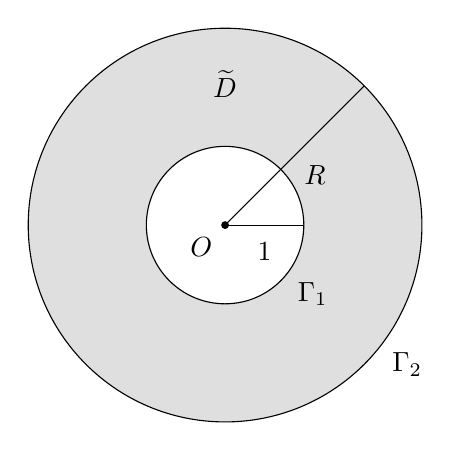
\begin{tikzpicture}
      \fill[gray!50,opacity=0.5] (0,0) circle (1) -- (0,0) circle (2.5);
      \fill[white] (0,0) circle (0.99);
      \draw (0,0) circle (1);
      \node[anchor=north west] at (0.8,-0.6) {$\Gamma_1$};
      \draw (0,0) circle (2.5);
      \node[anchor=north west] at (0 + 2.5 * 0.8, 0 - 2.5 * 0.6) {$\Gamma_2$};
      \node[fill,circle,inner sep=1pt,label=below left:$O$] at (0,0) {};
      \draw (0,0) -- (1,0);
      \node[anchor=north] at (0.5,-0.1) {$1$};
      \draw (0,0) -- (2.5 * 0.707, 2.5 * 0.707);
      \node[anchor=north west] at (2.5 * 0.707 / 2, 2.5 * 0.707 / 2) {$R$};
      \node[anchor=south] at (0,1.5) {$\widetilde{D}$};
    \end{tikzpicture}
  };
\end{tikzpicture}
\end{document}